\documentclass[]{article}
\usepackage{lmodern}
\usepackage{amssymb,amsmath}
\usepackage{ifxetex,ifluatex}
\usepackage{fixltx2e} % provides \textsubscript
\ifnum 0\ifxetex 1\fi\ifluatex 1\fi=0 % if pdftex
  \usepackage[T1]{fontenc}
  \usepackage[utf8]{inputenc}
\else % if luatex or xelatex
  \ifxetex
    \usepackage{mathspec}
  \else
    \usepackage{fontspec}
  \fi
  \defaultfontfeatures{Ligatures=TeX,Scale=MatchLowercase}
\fi
% use upquote if available, for straight quotes in verbatim environments
\IfFileExists{upquote.sty}{\usepackage{upquote}}{}
% use microtype if available
\IfFileExists{microtype.sty}{%
\usepackage{microtype}
\UseMicrotypeSet[protrusion]{basicmath} % disable protrusion for tt fonts
}{}
\usepackage[margin=1in]{geometry}
\usepackage{hyperref}
\hypersetup{unicode=true,
            pdftitle={Moisture Analysis},
            pdfborder={0 0 0},
            breaklinks=true}
\urlstyle{same}  % don't use monospace font for urls
\usepackage{color}
\usepackage{fancyvrb}
\newcommand{\VerbBar}{|}
\newcommand{\VERB}{\Verb[commandchars=\\\{\}]}
\DefineVerbatimEnvironment{Highlighting}{Verbatim}{commandchars=\\\{\}}
% Add ',fontsize=\small' for more characters per line
\usepackage{framed}
\definecolor{shadecolor}{RGB}{248,248,248}
\newenvironment{Shaded}{\begin{snugshade}}{\end{snugshade}}
\newcommand{\KeywordTok}[1]{\textcolor[rgb]{0.13,0.29,0.53}{\textbf{#1}}}
\newcommand{\DataTypeTok}[1]{\textcolor[rgb]{0.13,0.29,0.53}{#1}}
\newcommand{\DecValTok}[1]{\textcolor[rgb]{0.00,0.00,0.81}{#1}}
\newcommand{\BaseNTok}[1]{\textcolor[rgb]{0.00,0.00,0.81}{#1}}
\newcommand{\FloatTok}[1]{\textcolor[rgb]{0.00,0.00,0.81}{#1}}
\newcommand{\ConstantTok}[1]{\textcolor[rgb]{0.00,0.00,0.00}{#1}}
\newcommand{\CharTok}[1]{\textcolor[rgb]{0.31,0.60,0.02}{#1}}
\newcommand{\SpecialCharTok}[1]{\textcolor[rgb]{0.00,0.00,0.00}{#1}}
\newcommand{\StringTok}[1]{\textcolor[rgb]{0.31,0.60,0.02}{#1}}
\newcommand{\VerbatimStringTok}[1]{\textcolor[rgb]{0.31,0.60,0.02}{#1}}
\newcommand{\SpecialStringTok}[1]{\textcolor[rgb]{0.31,0.60,0.02}{#1}}
\newcommand{\ImportTok}[1]{#1}
\newcommand{\CommentTok}[1]{\textcolor[rgb]{0.56,0.35,0.01}{\textit{#1}}}
\newcommand{\DocumentationTok}[1]{\textcolor[rgb]{0.56,0.35,0.01}{\textbf{\textit{#1}}}}
\newcommand{\AnnotationTok}[1]{\textcolor[rgb]{0.56,0.35,0.01}{\textbf{\textit{#1}}}}
\newcommand{\CommentVarTok}[1]{\textcolor[rgb]{0.56,0.35,0.01}{\textbf{\textit{#1}}}}
\newcommand{\OtherTok}[1]{\textcolor[rgb]{0.56,0.35,0.01}{#1}}
\newcommand{\FunctionTok}[1]{\textcolor[rgb]{0.00,0.00,0.00}{#1}}
\newcommand{\VariableTok}[1]{\textcolor[rgb]{0.00,0.00,0.00}{#1}}
\newcommand{\ControlFlowTok}[1]{\textcolor[rgb]{0.13,0.29,0.53}{\textbf{#1}}}
\newcommand{\OperatorTok}[1]{\textcolor[rgb]{0.81,0.36,0.00}{\textbf{#1}}}
\newcommand{\BuiltInTok}[1]{#1}
\newcommand{\ExtensionTok}[1]{#1}
\newcommand{\PreprocessorTok}[1]{\textcolor[rgb]{0.56,0.35,0.01}{\textit{#1}}}
\newcommand{\AttributeTok}[1]{\textcolor[rgb]{0.77,0.63,0.00}{#1}}
\newcommand{\RegionMarkerTok}[1]{#1}
\newcommand{\InformationTok}[1]{\textcolor[rgb]{0.56,0.35,0.01}{\textbf{\textit{#1}}}}
\newcommand{\WarningTok}[1]{\textcolor[rgb]{0.56,0.35,0.01}{\textbf{\textit{#1}}}}
\newcommand{\AlertTok}[1]{\textcolor[rgb]{0.94,0.16,0.16}{#1}}
\newcommand{\ErrorTok}[1]{\textcolor[rgb]{0.64,0.00,0.00}{\textbf{#1}}}
\newcommand{\NormalTok}[1]{#1}
\usepackage{graphicx,grffile}
\makeatletter
\def\maxwidth{\ifdim\Gin@nat@width>\linewidth\linewidth\else\Gin@nat@width\fi}
\def\maxheight{\ifdim\Gin@nat@height>\textheight\textheight\else\Gin@nat@height\fi}
\makeatother
% Scale images if necessary, so that they will not overflow the page
% margins by default, and it is still possible to overwrite the defaults
% using explicit options in \includegraphics[width, height, ...]{}
\setkeys{Gin}{width=\maxwidth,height=\maxheight,keepaspectratio}
\IfFileExists{parskip.sty}{%
\usepackage{parskip}
}{% else
\setlength{\parindent}{0pt}
\setlength{\parskip}{6pt plus 2pt minus 1pt}
}
\setlength{\emergencystretch}{3em}  % prevent overfull lines
\providecommand{\tightlist}{%
  \setlength{\itemsep}{0pt}\setlength{\parskip}{0pt}}
\setcounter{secnumdepth}{0}
% Redefines (sub)paragraphs to behave more like sections
\ifx\paragraph\undefined\else
\let\oldparagraph\paragraph
\renewcommand{\paragraph}[1]{\oldparagraph{#1}\mbox{}}
\fi
\ifx\subparagraph\undefined\else
\let\oldsubparagraph\subparagraph
\renewcommand{\subparagraph}[1]{\oldsubparagraph{#1}\mbox{}}
\fi

%%% Use protect on footnotes to avoid problems with footnotes in titles
\let\rmarkdownfootnote\footnote%
\def\footnote{\protect\rmarkdownfootnote}

%%% Change title format to be more compact
\usepackage{titling}

% Create subtitle command for use in maketitle
\newcommand{\subtitle}[1]{
  \posttitle{
    \begin{center}\large#1\end{center}
    }
}

\setlength{\droptitle}{-2em}

  \title{Moisture Analysis}
    \pretitle{\vspace{\droptitle}\centering\huge}
  \posttitle{\par}
    \author{}
    \preauthor{}\postauthor{}
    \date{}
    \predate{}\postdate{}
  

\begin{document}
\maketitle

\begin{Shaded}
\begin{Highlighting}[]
\KeywordTok{library}\NormalTok{(psych)}

\CommentTok{# library}
\KeywordTok{library}\NormalTok{(ggplot2)}
\end{Highlighting}
\end{Shaded}

\begin{verbatim}
## 
## Attaching package: 'ggplot2'
\end{verbatim}

\begin{verbatim}
## The following objects are masked from 'package:psych':
## 
##     %+%, alpha
\end{verbatim}

\begin{Shaded}
\begin{Highlighting}[]
\KeywordTok{library}\NormalTok{(tidyverse)}
\end{Highlighting}
\end{Shaded}

\begin{verbatim}
## -- Attaching packages ----------------------------------------------------------------------------- tidyverse 1.2.1 --
\end{verbatim}

\begin{verbatim}
## v tibble  1.4.2     v purrr   0.2.5
## v tidyr   0.8.1     v dplyr   0.7.6
## v readr   1.1.1     v stringr 1.3.1
## v tibble  1.4.2     v forcats 0.3.0
\end{verbatim}

\begin{verbatim}
## -- Conflicts -------------------------------------------------------------------------------- tidyverse_conflicts() --
## x ggplot2::%+%()   masks psych::%+%()
## x ggplot2::alpha() masks psych::alpha()
## x dplyr::filter()  masks stats::filter()
## x dplyr::lag()     masks stats::lag()
\end{verbatim}

\begin{Shaded}
\begin{Highlighting}[]
\KeywordTok{library}\NormalTok{(data.table)}
\end{Highlighting}
\end{Shaded}

\begin{verbatim}
## 
## Attaching package: 'data.table'
\end{verbatim}

\begin{verbatim}
## The following objects are masked from 'package:dplyr':
## 
##     between, first, last
\end{verbatim}

\begin{verbatim}
## The following object is masked from 'package:purrr':
## 
##     transpose
\end{verbatim}

\begin{Shaded}
\begin{Highlighting}[]
\KeywordTok{library}\NormalTok{(GGally)}
\end{Highlighting}
\end{Shaded}

\begin{verbatim}
## 
## Attaching package: 'GGally'
\end{verbatim}

\begin{verbatim}
## The following object is masked from 'package:dplyr':
## 
##     nasa
\end{verbatim}

\begin{Shaded}
\begin{Highlighting}[]
\KeywordTok{library}\NormalTok{(lubridate)}
\end{Highlighting}
\end{Shaded}

\begin{verbatim}
## 
## Attaching package: 'lubridate'
\end{verbatim}

\begin{verbatim}
## The following objects are masked from 'package:data.table':
## 
##     hour, isoweek, mday, minute, month, quarter, second, wday,
##     week, yday, year
\end{verbatim}

\begin{verbatim}
## The following object is masked from 'package:base':
## 
##     date
\end{verbatim}

\begin{Shaded}
\begin{Highlighting}[]
\KeywordTok{library}\NormalTok{(readxl)}
\NormalTok{Isosuo_}\DecValTok{1}\NormalTok{ <-}\StringTok{ }\KeywordTok{read_excel}\NormalTok{(}\StringTok{"Data/Isosuo 11.7.-3.8_.xlsx"}\NormalTok{)}
\KeywordTok{names}\NormalTok{(Isosuo_}\DecValTok{1}\NormalTok{) <-}\StringTok{ }\KeywordTok{make.names}\NormalTok{(}\KeywordTok{names}\NormalTok{(Isosuo_}\DecValTok{1}\NormalTok{))}
\NormalTok{data_isosuo_weather <-}\StringTok{ }\NormalTok{Isosuo_}\DecValTok{1} \OperatorTok
\StringTok{  }\KeywordTok{rename}\NormalTok{(}\StringTok{"temp"}\NormalTok{=Temperature..C.) }\OperatorTok
\StringTok{  }\KeywordTok{rename}\NormalTok{(}\StringTok{"humid"}\NormalTok{=Humidity....)  }\OperatorTok
\StringTok{  }\KeywordTok{rename}\NormalTok{(}\StringTok{"timestamp"}\NormalTok{=}\StringTok{ }\NormalTok{Date.Time.Y.m.d.H.M.S.EEST..) }\OperatorTok\StringTok{ }
\StringTok{  }\KeywordTok{mutate}\NormalTok{(}\StringTok{"timestamp"}\NormalTok{=}\StringTok{ }\KeywordTok{ymd_hms}\NormalTok{(timestamp))}

\CommentTok{# setDT(myData)}
\CommentTok{# setDT(myData)[Isosuo_1, ch1, roll = "nearest", on = "timestamp"]}
\end{Highlighting}
\end{Shaded}

\begin{Shaded}
\begin{Highlighting}[]
\NormalTok{data_moisture <-}\StringTok{ }\KeywordTok{read.csv}\NormalTok{(}\StringTok{"./Data/AA2_data.csv"}\NormalTok{, }\DataTypeTok{sep =} \StringTok{";"}\NormalTok{) }\OperatorTok\StringTok{ }
\StringTok{  }\KeywordTok{rename}\NormalTok{(}\DataTypeTok{moisture1 =} \StringTok{"ch1"}\NormalTok{) }\OperatorTok\StringTok{ }
\StringTok{  }\KeywordTok{rename}\NormalTok{(}\DataTypeTok{moisture2 =} \StringTok{"Ch2"}\NormalTok{) }\OperatorTok\StringTok{ }
\StringTok{  }\KeywordTok{rename}\NormalTok{(}\DataTypeTok{moisture3 =} \StringTok{"Ch3"}\NormalTok{) }\OperatorTok\StringTok{ }
\StringTok{  }\KeywordTok{mutate}\NormalTok{(}\StringTok{"timestamp"}\NormalTok{=}\StringTok{ }\KeywordTok{ymd_hms}\NormalTok{(timestamp))}
\CommentTok{# testData <- myData[1:100, ]}
\end{Highlighting}
\end{Shaded}

\begin{Shaded}
\begin{Highlighting}[]
\NormalTok{data_ground_level_}\DecValTok{1}\NormalTok{ <-}\StringTok{ }\KeywordTok{read.csv}\NormalTok{(}\StringTok{"./Data/AA_2_1.csv"}\NormalTok{, }\DataTypeTok{sep =} \StringTok{";"}\NormalTok{) }\OperatorTok\StringTok{ }
\StringTok{  }\KeywordTok{select}\NormalTok{(}\StringTok{"X"}\NormalTok{, }\StringTok{"X.1"}\NormalTok{) }\OperatorTok\StringTok{ }
\StringTok{  }\KeywordTok{rename}\NormalTok{(}\DataTypeTok{timestamp =}\NormalTok{ X) }\OperatorTok
\StringTok{  }\KeywordTok{rename}\NormalTok{(}\DataTypeTok{water_height1 =}\NormalTok{ X.}\DecValTok{1}\NormalTok{) }\OperatorTok
\StringTok{  }\KeywordTok{slice}\NormalTok{(}\DecValTok{12}\OperatorTok{:}\KeywordTok{n}\NormalTok{())}

\NormalTok{data_ground_level_}\DecValTok{2}\NormalTok{ <-}\StringTok{ }\KeywordTok{read.csv}\NormalTok{(}\StringTok{"./Data/AA_2_2.csv"}\NormalTok{, }\DataTypeTok{sep =} \StringTok{";"}\NormalTok{) }\OperatorTok\StringTok{ }
\StringTok{  }\KeywordTok{select}\NormalTok{(}\StringTok{"X"}\NormalTok{, }\StringTok{"X.1"}\NormalTok{) }\OperatorTok\StringTok{ }
\StringTok{  }\KeywordTok{rename}\NormalTok{(}\DataTypeTok{timestamp =}\NormalTok{ X) }\OperatorTok
\StringTok{  }\KeywordTok{rename}\NormalTok{(}\DataTypeTok{water_height2 =}\NormalTok{ X.}\DecValTok{1}\NormalTok{) }\OperatorTok
\StringTok{  }\KeywordTok{slice}\NormalTok{(}\DecValTok{12}\OperatorTok{:}\KeywordTok{n}\NormalTok{())}

\NormalTok{data_ground_level_}\DecValTok{3}\NormalTok{ <-}\StringTok{ }\KeywordTok{read.csv}\NormalTok{(}\StringTok{"./Data/AA_2_3.csv"}\NormalTok{, }\DataTypeTok{sep =} \StringTok{";"}\NormalTok{) }\OperatorTok\StringTok{ }
\StringTok{  }\KeywordTok{select}\NormalTok{(}\StringTok{"X"}\NormalTok{, }\StringTok{"X.1"}\NormalTok{) }\OperatorTok\StringTok{ }
\StringTok{  }\KeywordTok{rename}\NormalTok{(}\DataTypeTok{timestamp =}\NormalTok{ X) }\OperatorTok
\StringTok{  }\KeywordTok{rename}\NormalTok{(}\DataTypeTok{water_height3 =}\NormalTok{ X.}\DecValTok{1}\NormalTok{) }\OperatorTok
\StringTok{  }\KeywordTok{slice}\NormalTok{(}\DecValTok{12}\OperatorTok{:}\KeywordTok{n}\NormalTok{()) }

\CommentTok{# TO DO: convert to timestamp}
  \CommentTok{#mutate(timestamp = as.time)}

\KeywordTok{summary}\NormalTok{(data_ground_level_}\DecValTok{3}\NormalTok{)}
\end{Highlighting}
\end{Shaded}

\begin{verbatim}
##                timestamp     water_height3  
##                     :    8   -47    :10521  
##  01.07.2018 00:00:00:    1   -46    :10401  
##  01.07.2018 00:05:00:    1   -48    :  918  
##  01.07.2018 00:10:00:    1   133    :  152  
##  01.07.2018 00:15:00:    1   414    :  120  
##  01.07.2018 00:20:00:    1   121    :  115  
##  (Other)            :27599   (Other): 5385
\end{verbatim}

\begin{Shaded}
\begin{Highlighting}[]
\NormalTok{data_ground_level <-}\StringTok{ }\KeywordTok{inner_join}\NormalTok{(data_ground_level_}\DecValTok{1}\NormalTok{, data_ground_level_}\DecValTok{2}\NormalTok{, }\DataTypeTok{by=}\StringTok{"timestamp"}\NormalTok{)}
\end{Highlighting}
\end{Shaded}

\begin{verbatim}
## Warning: Column `timestamp` joining factors with different levels, coercing
## to character vector
\end{verbatim}

\begin{Shaded}
\begin{Highlighting}[]
\NormalTok{data_ground_level <-}\StringTok{ }\KeywordTok{inner_join}\NormalTok{(data_ground_level, data_ground_level_}\DecValTok{3}\NormalTok{, }\DataTypeTok{by=}\StringTok{"timestamp"}\NormalTok{)}
\end{Highlighting}
\end{Shaded}

\begin{verbatim}
## Warning: Column `timestamp` joining character vector and factor, coercing
## into character vector
\end{verbatim}

\begin{Shaded}
\begin{Highlighting}[]
  \CommentTok{# }\AlertTok{TODO}\CommentTok{: convert to timestamp}
  \CommentTok{#mutate("timestamp"= str_replace(., ".", "-"))}

\CommentTok{#TODO check the join is correct. What happened to missing measurements. Why there is more data}
\end{Highlighting}
\end{Shaded}

\begin{Shaded}
\begin{Highlighting}[]
\NormalTok{data_combined <-}\StringTok{ }\KeywordTok{inner_join}\NormalTok{(data_isosuo_weather, data_moisture, }\DataTypeTok{by=}\StringTok{"timestamp"}\NormalTok{)}
\end{Highlighting}
\end{Shaded}

\section{Overview of Data}\label{overview-of-data}

\begin{Shaded}
\begin{Highlighting}[]
\KeywordTok{head}\NormalTok{(data_combined)}
\end{Highlighting}
\end{Shaded}

\begin{verbatim}
## # A tibble: 6 x 13
##   timestamp            temp X2nd.TempTemper~ Wind.speed..m.s.
##   <dttm>              <dbl>            <dbl>            <dbl>
## 1 2018-07-29 10:23:53  23.8             18.7              2.8
## 2 2018-07-29 10:28:53  23.9             18.7              3.1
## 3 2018-07-29 10:33:53  24               18.7              2.8
## 4 2018-07-29 10:53:53  25               18.7              1.4
## 5 2018-07-29 10:58:53  24.8             18.7              2.5
## 6 2018-07-29 11:03:53  24.8             18.7              1.7
## # ... with 9 more variables: Wind.gust..m.s. <dbl>,
## #   Wind.direction..deg. <dbl>, humid <dbl>, Rainfall..mm. <dbl>,
## #   Solar.radiation..W.m.2. <dbl>, Pressure..hPa. <dbl>, moisture1 <dbl>,
## #   moisture2 <dbl>, moisture3 <dbl>
\end{verbatim}

\begin{Shaded}
\begin{Highlighting}[]
\KeywordTok{describe}\NormalTok{(data_combined)}
\end{Highlighting}
\end{Shaded}

\begin{verbatim}
## Warning in FUN(newX[, i], ...): no non-missing arguments to min; returning
## Inf
\end{verbatim}

\begin{verbatim}
## Warning in FUN(newX[, i], ...): no non-missing arguments to max; returning
## -Inf
\end{verbatim}

\begin{verbatim}
##                          vars  n    mean     sd  median trimmed    mad
## timestamp                   1 71     NaN     NA      NA     NaN     NA
## temp                        2 71   27.77   1.36   28.20   28.01   1.04
## X2nd.TempTemperature..C.    3 71   19.80   0.72   20.00   19.82   0.74
## Wind.speed..m.s.            4 71    2.90   0.65    2.80    2.86   0.44
## Wind.gust..m.s.             5 71    5.06   0.96    5.30    5.06   0.89
## Wind.direction..deg.        6 71  125.79  11.14  127.00  126.09  11.86
## humid                       7 71   43.79  10.35   40.90   42.32   5.78
## Rainfall..mm.               8 71    0.00   0.00    0.00    0.00   0.00
## Solar.radiation..W.m.2.     9 71  457.66 145.85  485.00  465.09 174.95
## Pressure..hPa.             10 71 1023.74   0.72 1023.50 1023.64   0.59
## moisture1                  11 71   16.44   0.00   16.44   16.44   0.00
## moisture2                  12 71   16.44   0.00   16.44   16.44   0.00
## moisture3                  13 71   25.65   0.10   25.69   25.64   0.20
##                              min     max  range  skew kurtosis    se
## timestamp                    Inf    -Inf   -Inf    NA       NA    NA
## temp                       23.80   29.20   5.40 -1.42     1.23  0.16
## X2nd.TempTemperature..C.   18.70   21.00   2.30 -0.21    -1.37  0.09
## Wind.speed..m.s.            1.40    5.00   3.60  0.52     0.63  0.08
## Wind.gust..m.s.             2.80    7.50   4.70 -0.01    -0.38  0.11
## Wind.direction..deg.       95.00  147.00  52.00 -0.28    -0.27  1.32
## humid                      30.80   71.00  40.20  1.20     0.60  1.23
## Rainfall..mm.               0.00    0.00   0.00   NaN      NaN  0.00
## Solar.radiation..W.m.2.   182.00  653.00 471.00 -0.32    -1.23 17.31
## Pressure..hPa.           1022.90 1025.50   2.60  1.05     0.08  0.09
## moisture1                  16.44   16.44   0.00   NaN      NaN  0.00
## moisture2                  16.44   16.44   0.00   NaN      NaN  0.00
## moisture3                  25.55   25.83   0.28  0.47    -1.14  0.01
\end{verbatim}

\section{Plots}\label{plots}

\subsection{Histogram}\label{histogram}

\begin{Shaded}
\begin{Highlighting}[]
\CommentTok{# Basic histogram}
\KeywordTok{ggplot}\NormalTok{(data_combined, }\KeywordTok{aes}\NormalTok{(}\DataTypeTok{x=}\NormalTok{moisture1)) }\OperatorTok{+}\StringTok{ }\KeywordTok{geom_histogram}\NormalTok{(}\DataTypeTok{binwidth =} \FloatTok{0.005}\NormalTok{)}
\end{Highlighting}
\end{Shaded}

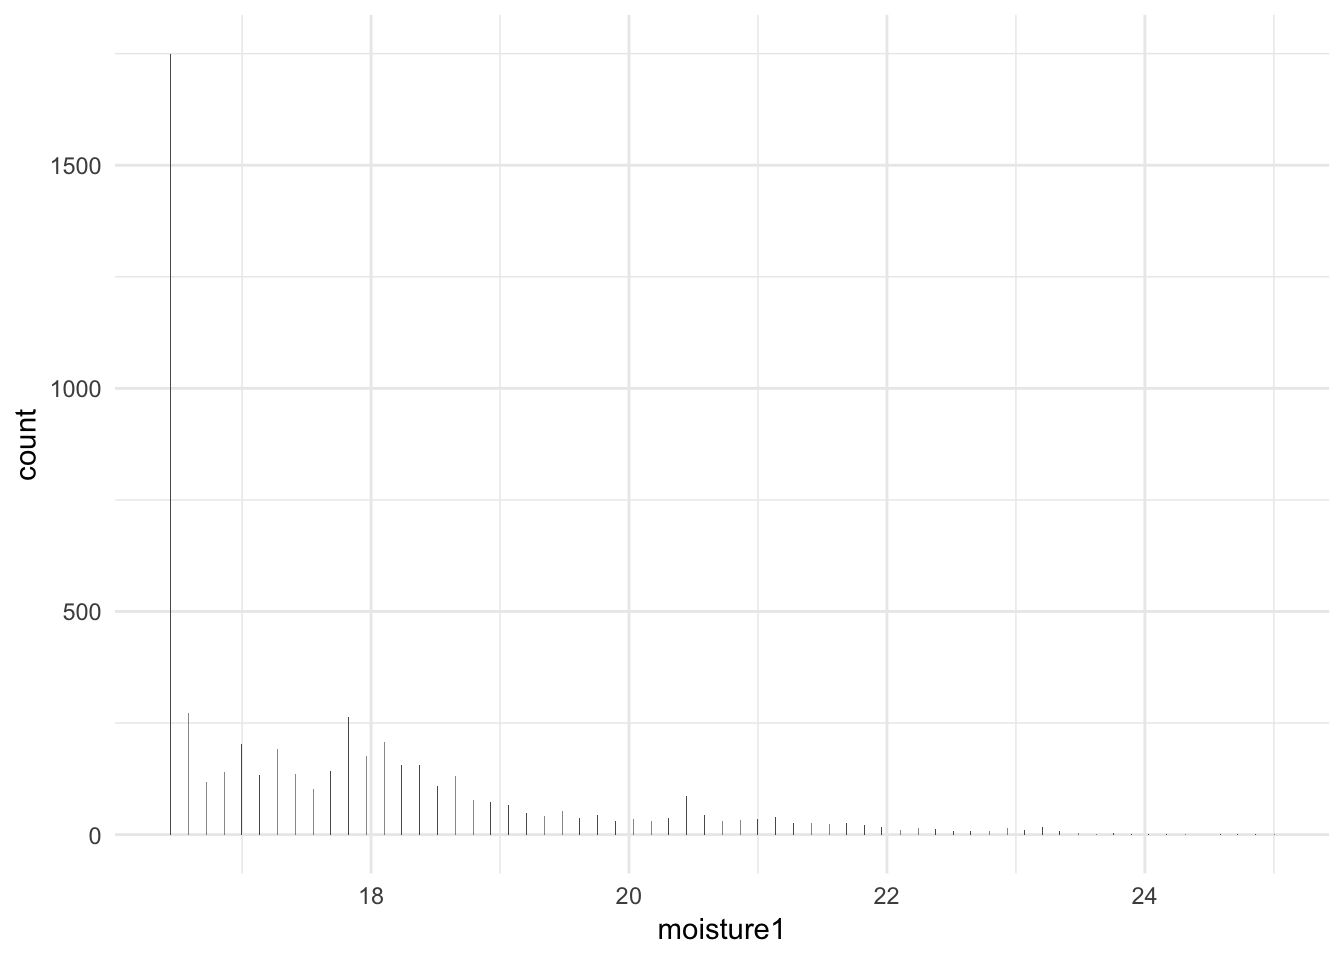
\includegraphics{output_files/figure-latex/histogram-1.pdf}

\begin{Shaded}
\begin{Highlighting}[]
\KeywordTok{ggplot}\NormalTok{(data_combined, }\KeywordTok{aes}\NormalTok{(}\DataTypeTok{x=}\NormalTok{moisture2)) }\OperatorTok{+}\StringTok{ }\KeywordTok{geom_histogram}\NormalTok{()}
\end{Highlighting}
\end{Shaded}

\begin{verbatim}
## `stat_bin()` using `bins = 30`. Pick better value with `binwidth`.
\end{verbatim}

\begin{verbatim}
## Warning: Computation failed in `stat_bin()`:
## `binwidth` must be positive
\end{verbatim}

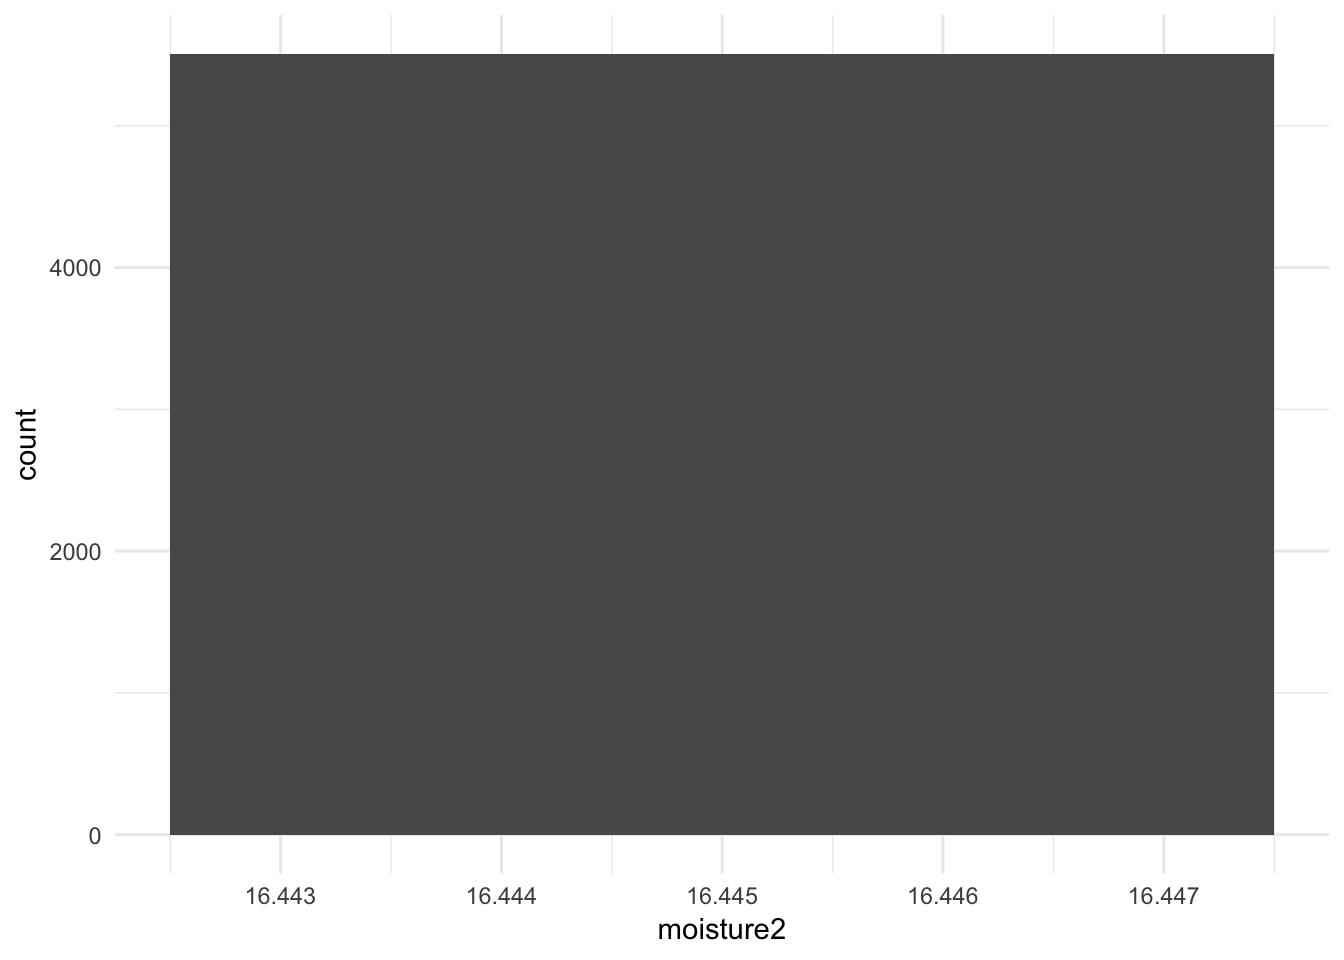
\includegraphics{output_files/figure-latex/histogram-2.pdf}

\begin{Shaded}
\begin{Highlighting}[]
\CommentTok{# Custom Binning. I can just give the size of the bin}
\KeywordTok{ggplot}\NormalTok{(data_combined, }\KeywordTok{aes}\NormalTok{(}\DataTypeTok{x=}\NormalTok{moisture3)) }\OperatorTok{+}\StringTok{ }\KeywordTok{geom_histogram}\NormalTok{(}\DataTypeTok{binwidth =} \FloatTok{0.00001}\NormalTok{)}
\end{Highlighting}
\end{Shaded}

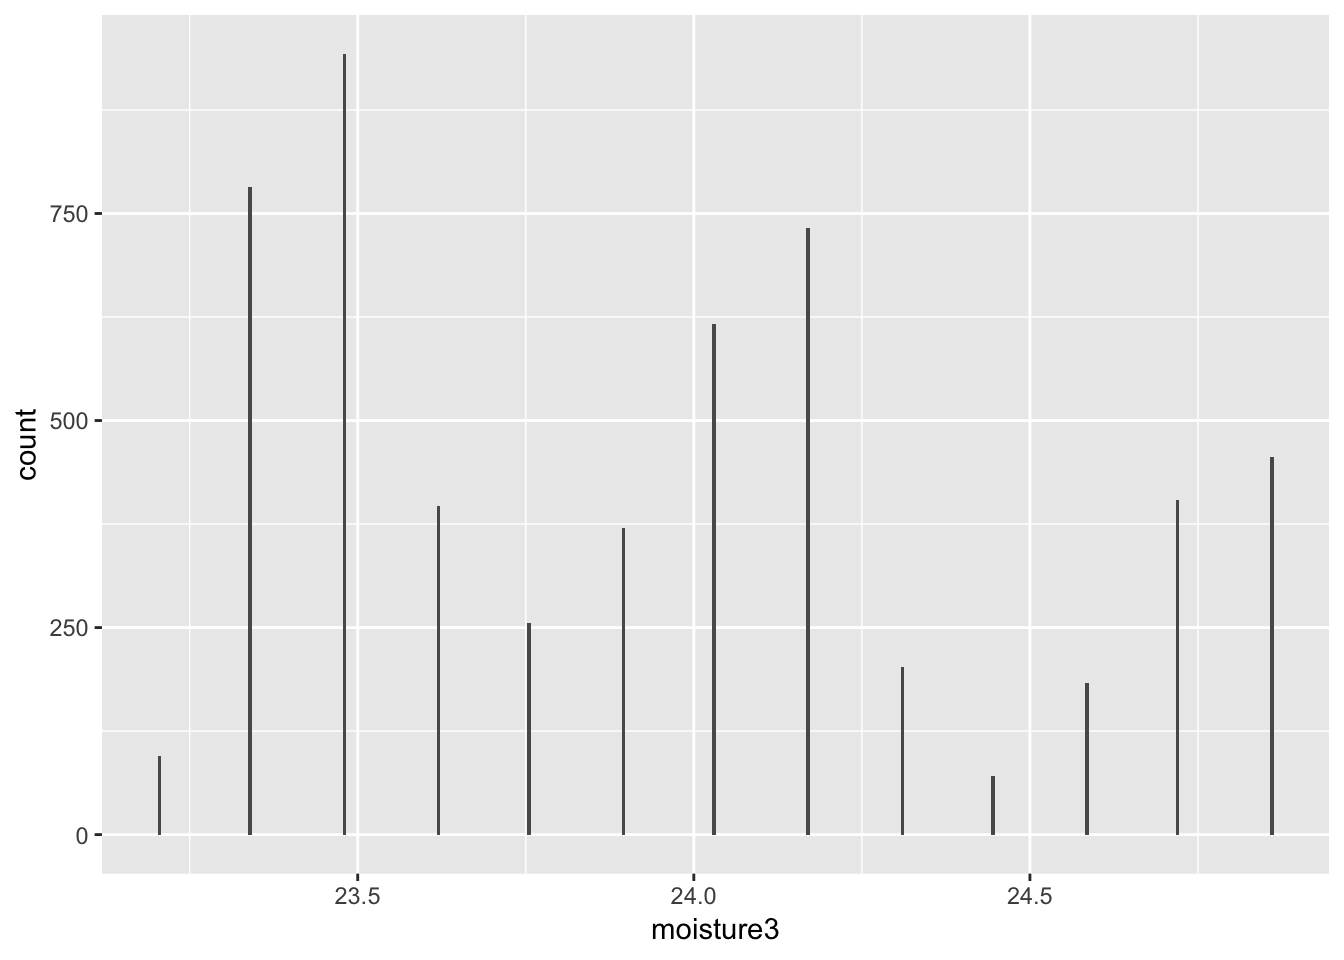
\includegraphics{output_files/figure-latex/histogram-3.pdf} \#\#
Scatterplots

\begin{Shaded}
\begin{Highlighting}[]
\CommentTok{# basic scatterplot}
\KeywordTok{ggplot}\NormalTok{(data_combined, }\KeywordTok{aes}\NormalTok{(}\DataTypeTok{x=}\NormalTok{timestamp, }\DataTypeTok{y=}\NormalTok{moisture3)) }\OperatorTok{+}\StringTok{ }
\StringTok{  }\KeywordTok{geom_point}\NormalTok{()}
\end{Highlighting}
\end{Shaded}

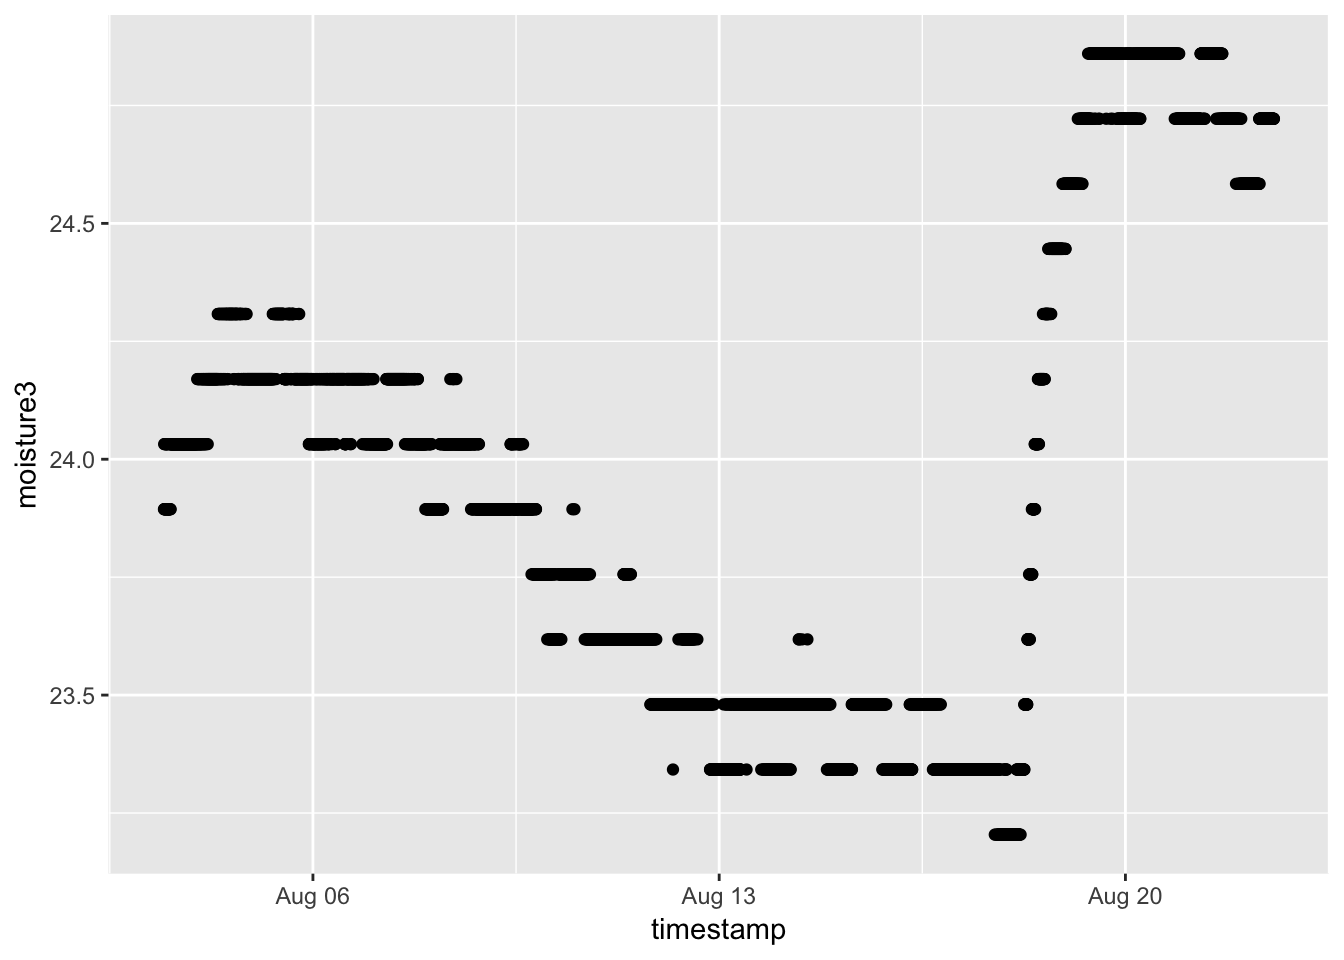
\includegraphics{output_files/figure-latex/scatterplots-1.pdf}

\begin{Shaded}
\begin{Highlighting}[]
\CommentTok{# Custom Binning. I can just give the size of the bin}
\KeywordTok{ggplot}\NormalTok{(data_combined, }\KeywordTok{aes}\NormalTok{(}\DataTypeTok{x=}\NormalTok{temp)) }\OperatorTok{+}\StringTok{ }\KeywordTok{geom_histogram}\NormalTok{(}\DataTypeTok{binwidth =} \FloatTok{0.05}\NormalTok{)}
\end{Highlighting}
\end{Shaded}

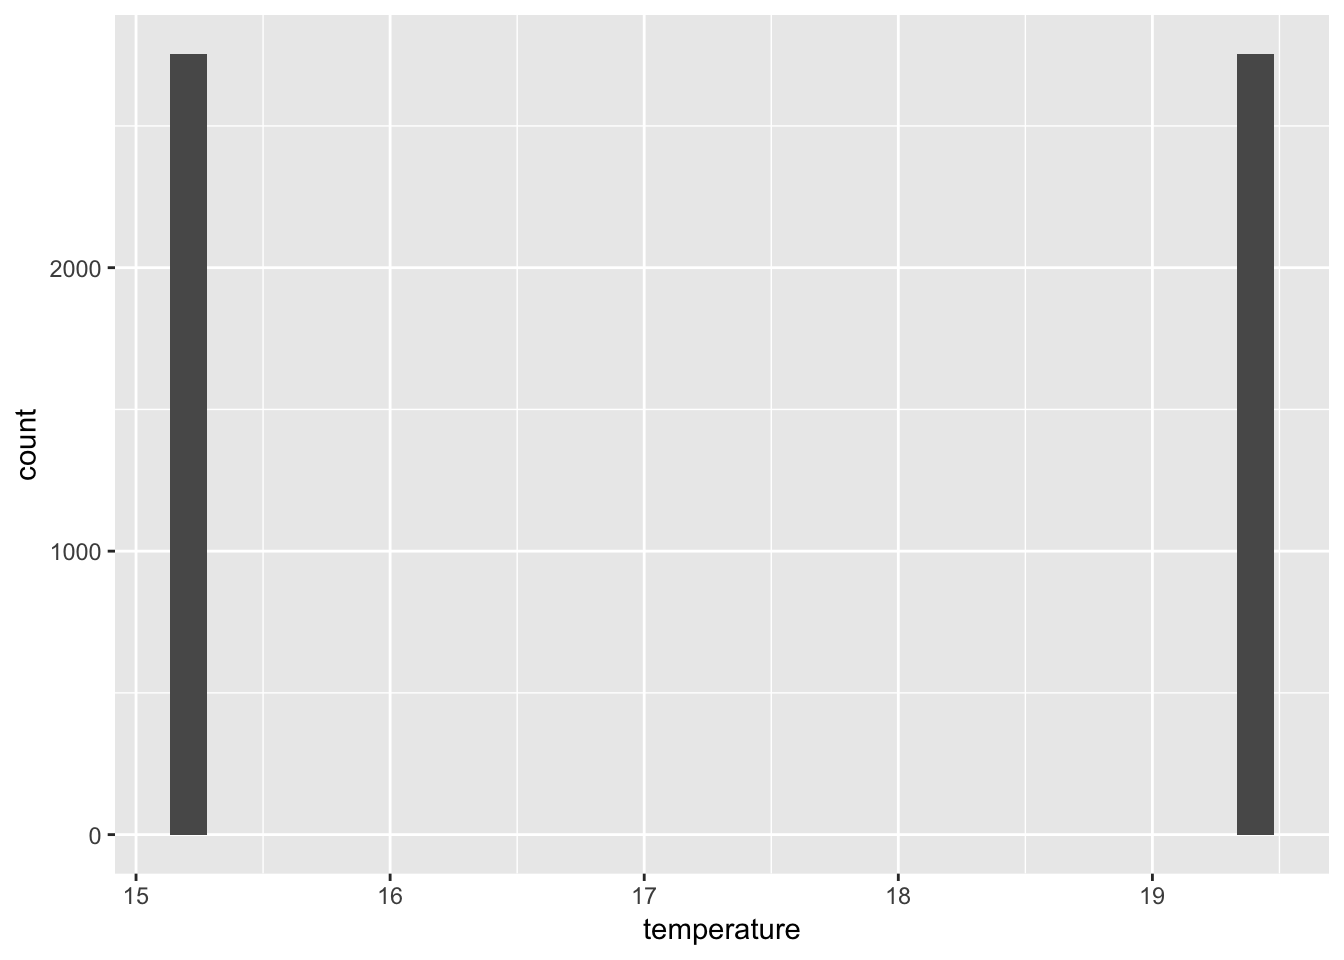
\includegraphics{output_files/figure-latex/plotXls_iso-1.pdf}

\begin{Shaded}
\begin{Highlighting}[]
\KeywordTok{ggpairs}\NormalTok{(data_combined, }\DataTypeTok{columns=}\KeywordTok{c}\NormalTok{(}\StringTok{"temp"}\NormalTok{, }\StringTok{"Wind.gust..m.s."}\NormalTok{, }\StringTok{"humid"}\NormalTok{, }\StringTok{"moisture1"}\NormalTok{, }\StringTok{"moisture2"}\NormalTok{, }\StringTok{"moisture3"}\NormalTok{))}
\end{Highlighting}
\end{Shaded}

\begin{verbatim}
## Warning in cor(x, y, method = method, use = use): the standard deviation is
## zero

## Warning in cor(x, y, method = method, use = use): the standard deviation is
## zero

## Warning in cor(x, y, method = method, use = use): the standard deviation is
## zero

## Warning in cor(x, y, method = method, use = use): the standard deviation is
## zero

## Warning in cor(x, y, method = method, use = use): the standard deviation is
## zero

## Warning in cor(x, y, method = method, use = use): the standard deviation is
## zero

## Warning in cor(x, y, method = method, use = use): the standard deviation is
## zero

## Warning in cor(x, y, method = method, use = use): the standard deviation is
## zero

## Warning in cor(x, y, method = method, use = use): the standard deviation is
## zero
\end{verbatim}

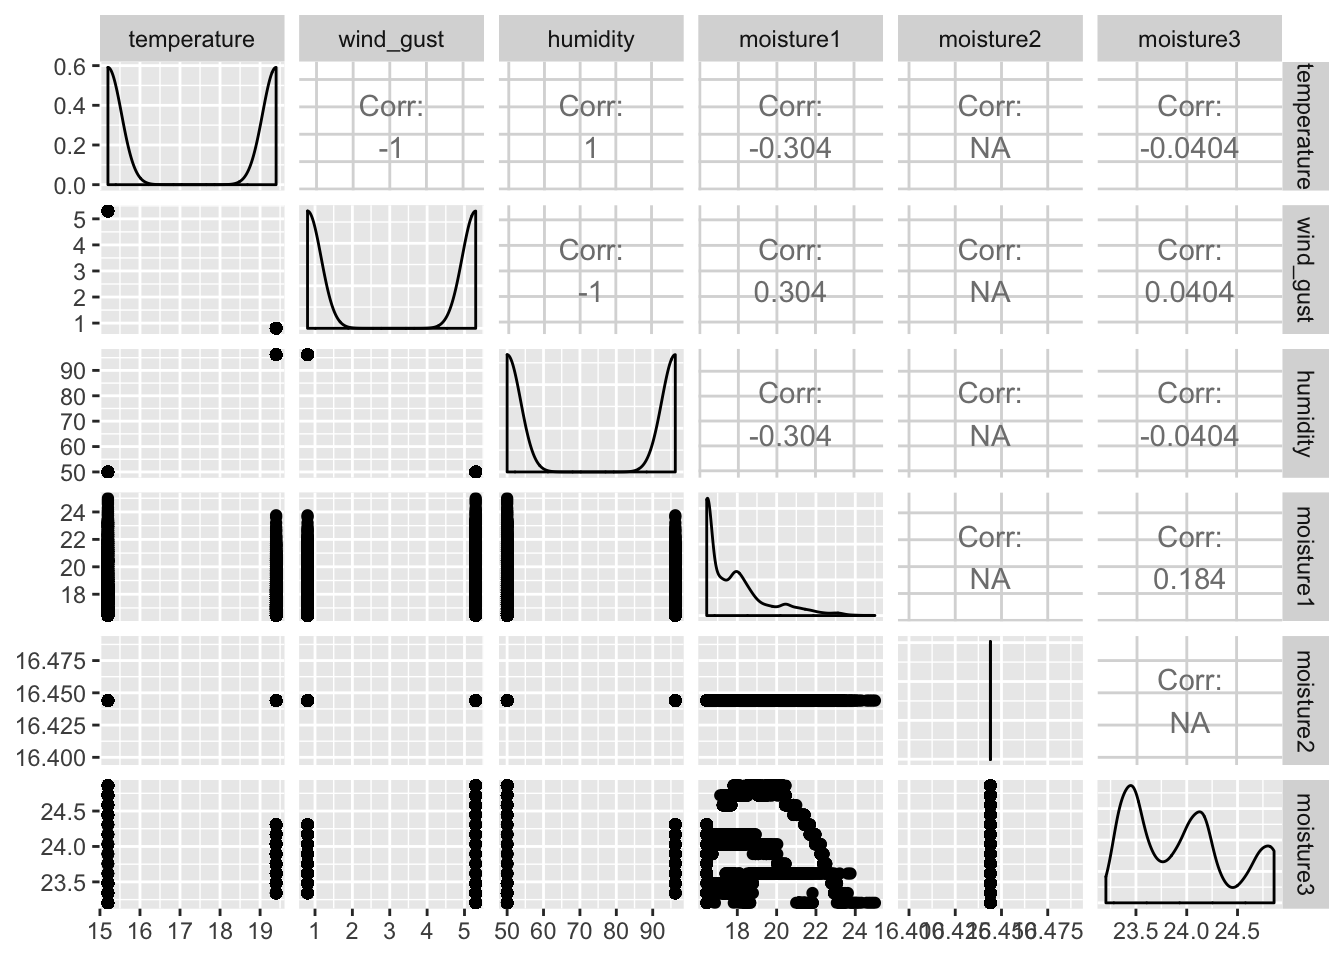
\includegraphics{output_files/figure-latex/plotPairs-1.pdf}


\end{document}
